\documentclass[conference]{IEEEtran}
% Some Computer Society conferences also require the compsoc mode option,
% but others use the standard conference format.
%

\usepackage[pdftex]{graphicx}
\graphicspath{{./Figures}}

% *** CITATION PACKAGES ***
%
%\usepackage{cite}
% cite.sty was written by Donald Arseneau

\usepackage{comment}
\usepackage{mcite}
\usepackage{cancel}
\usepackage{blkarray}
\usepackage[export]{adjustbox}
\usepackage{tikz}
\usepackage[mode=buildnew]{standalone}% requires -shell-escape
\usepackage{pgfplots, pgfplotstable}
\pgfplotsset{compat=1.16}
\usepackage{lipsum}
\usepackage{colortbl}
\usepackage{hyperref}
\usepackage{graphicx}
\graphicspath{ {figs/} }

\newcommand{\francisco}[1]  {\textbf{\textcolor{blue}{[Francisco] #1}}}
\newcommand{\nath}[1]{\textcolor{green}{#1} }

% *** MATH PACKAGES ***
%
\usepackage{amsmath}

% *** SUBFIGURE PACKAGES ***
\ifCLASSOPTIONcompsoc
  \usepackage[caption=false,font=normalsize,labelfont=sf,textfont=sf]{subfig}
\else
  \usepackage[caption=false,font=footnotesize]{subfig}
\fi

\begin{document}
\bstctlcite{IEEEexample:BSTcontrol}

%\title{ThingSat, Case Study for In-Orbit Firmware and Software Updates Architecture}
\title{ThingSat: Low-Power Secure CubeSat Software Updates
over Ground-Flight Communications}

% author names and affiliations
% use a multiple column layout for up to three different
% affiliations
\author{
%\IEEEauthorblockN{J. Kirk, H. Simpson and M. Scott}
\IEEEauthorblockN{Authors}
\IEEEauthorblockA{Something, France.
Email: first.lastname@something.fr}}

% make the title area
\maketitle

% As a general rule, do not put math, special symbols or citations
% in the abstract
\begin{abstract}
TO DO.
\end{abstract}

\IEEEpeerreviewmaketitle

\section{Introduction}
\label{sec:introduction}

Driven in part by the increasing involvement from public research and the academic
community~\cite{cubesat101}, more and more open source software and hardware is available,
maturing and used on CubeSats.

Their availability has lowered the bar of entry, with the aim of designing low-cost
CubeSats which can more reliably achieve a successful launch -- until recently, the
failure rate was still around 60\% for first-time satellite builders~\cite{Holliday2019PyCubed}.

With the same objective, another trend has been to buy tiny "rack-space" in
orbit~\cite{satrevolution2020}. With this model, a stakeholder (a user) can place
a small ($<$1U) payload slot hosted inside a CubeSat provided by an operator
(a different stakeholder). The user only needs to design and operate this payload,
instead of designing and operating the whole CubeSat, drastically reducing users'
costs and lead time. Typically, such a payload boils down to a printed circuit board
(PCB) with sensors, a low-power CPU (sometimes with separate wireless communication
capabilities) and a bus communication interface to the CubeSat main on-board flight
computer (OBC). As such, a hosted payload on a CubeSat resembles small embedded
devices usually found in the Internet of Things (IoT).

Nevertheless, even if the entry bar is lowered through the combination of a hosted payload
and leveraging open source, software embarked on launched CubeSats tend to be
minimalist (think: space rush, time pressure to meet hard launch deadlines...)
and buggy, as most software is. In effect, hosted CubeSat payload software must
typically be updated over-the-air (OTA) regularly, after it is deployed in orbit
and in operation. Beyond enabling OTA software updates on a hosted CubSat payload,
cybersecurity is a crucial emerging aspect. Indeed, on the one hand, software
updates can be used to fix vulnerabilities but, on the other hand, tampering with
software updates can be used as a cyberattack vector~\cite{ccleaner}.

State-of-the-art has so far focused on single-stakeholder CubeSats use cases,
where embarked software is managed by a single entity. In this paper, we instead
focus on the challenge of securing software updates on low-cost multi-tenant CubeSats
whereby the OBC and the payload are operated by different stakeholders which do not
necessarily trust each other. In particular, we focus on payloads based on low-power
microcontrollers, which are essential on low-cost CubeSats, where
low power consumption is a key factor.

\section{Background \& Related Work} 
\label{sec:background-related-work}

\subsection{CubeSat} 
\label{sec:cubesat}

\subsection{Cube Sat Protocol (CSP)} 
\label{sec:csp}

\paragraph*{Architecture}
% - electronics
% - connectivity
% - payloads, obc, etc..

\subsection{Open Source} \cite{shalashov2021OpenSourceCubeSatReview}, \cite{Holliday2019PyCubedAO}
\paragraph*{Why Open-Source Satellite Initiatives}
\paragraph*{pyCube, etc.}
% - overview of alternatives
% - hardware software overview

\subsection{LoRa} \cite{saeed2020CubeSatReview} 
\label{sec:lora-cubesat}
\paragraph*{CubeSat LoRa missions}
\paragraph*{Research topics, challenges of LoRa in space}

\subsection{RIOT} \cite{baccelli2018riot}
\paragraph{Overview of the Project}
\paragraph{Overview of the architecture}

\section{Case Study: ThingSat}
\label{sec:case-study}

The ThingSat project~\cite{git:thingsat-repo} aims to benchmark ground-space
LoRa links on different frequency bands and demonstrate the
effectiveness of that technology inside a LEO (Low Earth Orbit) CubeSat.

ThingSat is deployed as a hosted payload on a shared 3U CubeSat:
\href{https://space.skyrocket.de/doc_sdat/stork-1.htm}{STORK-1} from the polish
start-up \href{https://www.satrevolution.com/}{SatRevolution}. The CubeSat was
launched on January 13th, 2022,currently in orbit at an altitude of 525 km (see its
\href{https://www.n2yo.com/database/?q=STORK-1\#results}{Two-Line Elements}).

The ThingSat payload now in orbit is used for Ocean level monitoring. However,
its design can be adequate for a wider variety of use cases, in Earth science
academic research (e.g. tacking the  melting of glaciers, pirate fishing...)
and in the industry for companies using geographically dispersed devices (e.g.
monitoring of tank ships...).

\begin{figure}[t]
\centering
    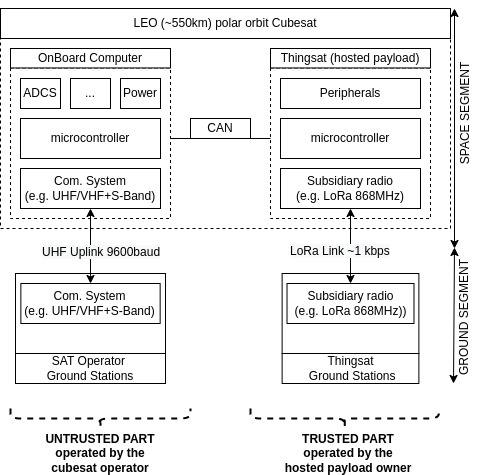
\includegraphics[width=0.35\textwidth]{Figures/globecom-thingsat-mods.jpg}
    \caption{ThingSat hosted payload: deployed components and architecture.}
    \label{fig:thingsat-archi}
\end{figure}

\subsection{Distributed System Architecture}
\label{sec:thingsat-hw}
\autoref{fig:thingsat-archi} describes the ThingSat deployment components, it gives an
overview of a typical CubeSat ecosystem, whereby the interaction with this payload
traverses untrusted elements.

\subsection*{Low-power Space Segment}
The Space Segment comprises the on-board computer (OBC) and hosted payloads, whom,
interconnected via a CAN bus, which share resources on the CubeSat.
\begin{itemize}
\item The OBC provided by the satellite operator consists on
a microcontroller with all its subsystems to operate the CubeSat:
Attitude Determination and Control System (ADCS),
communication subsystems (UHF/VHF/S-band for uplink/downlink and antennas) and
power subsystem (Battery Management, Energy Harvesting with Solar Panels, Auxiliary Power Supply).

\item We designed the ThingSat payload, using a STM32F405RG %STM32F446RE
microcontroller featuring an ARM Cortex-M4 core
and open source firmware based on RIOT~\cite{baccelli2018riot}. The ThingSat payload embeds both a
\href{https://www.semtech.com/products/wireless-rf/lora-gateways/sx1302}{Semtech SX1302 transceiver} for
communications on the 863\-870 MHz band and a \href{https://www.semtech.com/products/wireless-rf/24-ghz-transceivers/sx1280}{Semtech SX1280 transceiver}
for communications on the 2400\-2500 MHz band. Furthermore we designed a corresponding dual-band patch antenna (868MHz, 2.4GHz).
When active and using the 863\-870 MHz band, the ThingSat payload consumes at 3.3V:
(i) 90 mA in standby,
(ii) 110 mA during a frame reception (RX) and
(iii) 300 mA during a frame transmission (TX) at 27 dBm.
\end{itemize}

\subsection*{Ground Segments}
Ground Segment elements that communicate with the ThingSat payload are:
\begin{itemize}
\item \textbf{SatRevolution Ground Stations}: provided by the CubeSat operator \footnote{not
necessarily owned by the CubeSat operator} to communicate via UHF/VHF with the OBC,
and indirectly with the payload. This can be done directly od through a Command \&
Control Center, which acts as a broker between payload maintainers and hosted payload
(indirect access).
\item \href{https://github.com/thingsat/tinygs_2g4station}{\textbf{ThingSat LoRa Ground Stations}}:
that we designed, deployed and maintain, which can communicate via LoRa \textbf{directly} with the
ThingSat payload. These stations are based on an ESP32 microcontroller, and a 2.4GHz SX1280-LoRa
transceiver, also running an open source firmware based on RIOT.
\end{itemize}

\subsection{Communication Characteristics Overview}
\label{sec:thingsat-comm-characteristics}

ThingSat payload communicates either directly via low-power WAN, or indirectly
via the UHF/VHF link provided by the CubeSat's OBC.

\paragraph*{Direct communication patterns via low-power WAN}
ThingSat can communicate directly with LoRa. In principle, although it is not used as
such so far, this communication link could also be used to transport software updates.
As shown in \autoref{fig:thingsat-comm} the ThingSat payload may act as either:
(i) a Sat-IoT end-device (ED) that will send LoRa frames to terrestrial LoRaWAN gateways or ThingSat ground stations (GS), or
(ii) an in-orbit LoRa sniffer, or
(iii) a store-carry-and-forward LoRa gateway.

Patterns (i) and (ii) allow to benchmark simple ground-space LoRa links by
computing statistics over multiple sent/received frames.
Pattern (iii) is a more
complex scenario: the satellite stores packets received from GS/ED and deliver
them once GS/ED destinations are inside the footprint of the satellite.

\paragraph*{Indirect communication characteristics via UHF/VHF}
CubeSat-GS communications are typically done on amateur frequency
bands (UHF/VHF) with typically low data rates ranging from 9.6kbps to
100kbps.
A polar LEO satellite will typically pass over a given ground station 2 to 4 times/day,
each pass having a communication window of to 10 minutes.

For ThingSat, the CubeSat Operator provides only 2 ground stations (both in Europe), communicating with
the CubeSat via a 10-kbps UHF/VHF link. Thus, the daily throughput is roughly
1500KB (corresponding to 2 GS x 2 passes/day x 5-min pass duration x 10Kbps).
However, this throughput must be shared between communications to/from the OBC
(for telecommand/telemetry/update) and to/from hosted payloads. Therefore in practice,
the total communication budget available for ThingSat via the UHF/VHF link is around
300KB/day.

\paragraph*{Intermittent communication/power supply}
Last but not least, the ThingSat payload is not constantly powered on. Typically, at point any time,
only a single hosted payload is powered on. For a 3U, 1U is dedicated to the OBC
and the remaining 2U, available for hosted payloads (8 payloads slots of 0.25U
in the case of ThingSat). Therefore, on average ThingSat is powered only 1/8th (12.5\%) of the time
(modulo other factors such as mission specificities, regulations, battery level etc.).

\subsection{Hosted Payload Software Updates Requirements}
\label{sec:thingsat-update-req}
Data exchanges between the Payload Maintainer and ThingSat consist on
\textbf{downlinks}: used by ThingSat to send mission results (radio metadata, frame stats, collected LoRa frames)
and diagnosis data (debug info on failed missions/updates)l \textbf{uplinks}: used for software updates of two categories:
\begin{enumerate}
    \item Firmware updates: to fix bugs, add/improve functionality (typically $\sim 200kB$ per FW, 1 FW/month);
    \item Mission updates: to configure scenarios (typically $\sim 700B$ per mission scenario, 1 scenario/day);
\end{enumerate}

\begin{figure}[t]
    \centering
    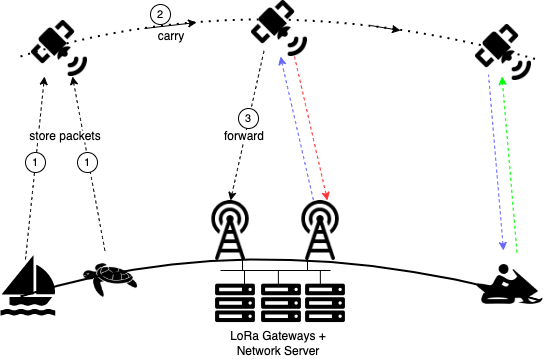
\includegraphics[width=0.4\textwidth]{Figures/thingsat-dtn.png}
    \caption{ThingSat in-orbit communication patterns.}
    \label{fig:thingsat-comm}
\end{figure}

\section{Cubedate: Standard Security for Continuous Deployment of Low-power CubeSat Software}
\label{sec:low-power-orbital-communication-arch}


The minimal security guarantees that we aim for are authenticity and integrity of software udpates, during the lifetime of the satellite mission.
These guarantees must remain valid end-to-end, all the way from the hosted payload software maintainer to the payload hosted in orbit on the CubeSat.
The basic process we use for securing authenticity and integrity of software udpates is decomposed in six phases shown \autoref{fig:phases}. 

\subsection{Basic Software Life-cycle Phases}

During a preliminary, pre-flight phase (\textit{Phase 0}) the authorized maintainer for the CubeSat-hosted payload
produces and flashes the payload with commissioning material:
a bootloader, the initial firmware, and authorized crypto material (a public key, and a crypographically strong hash function).
Once the hosted payload is commissioned it can be sent to the CubeSat operator of installation in the CubeSat.


Once the CubeSat in orbit, the hosted payload maintainer can trigger iterations through cycles of Phases 1-5, whereby
the authorized maintainer can build a new software update (\textit{Phase 1}), hash the update
and sign the hash (\textit{Phase 2}) then push a network transfer (PUT) towards the hosted payload via the ground station and the OBC (\textit{Phase 3.1}). The next time it wakes up, the hosted payload can
then ping and fetch (GET) the update from the OBC (\textit{Phase 3.2}), proceed to verify the signature and the hash (\textit{Phase 4}),
and upon successful verification, install/boot the new software (\textit{Phase 5}), otherwise the update is dropped.

\begin{figure}[t]
    \centering
    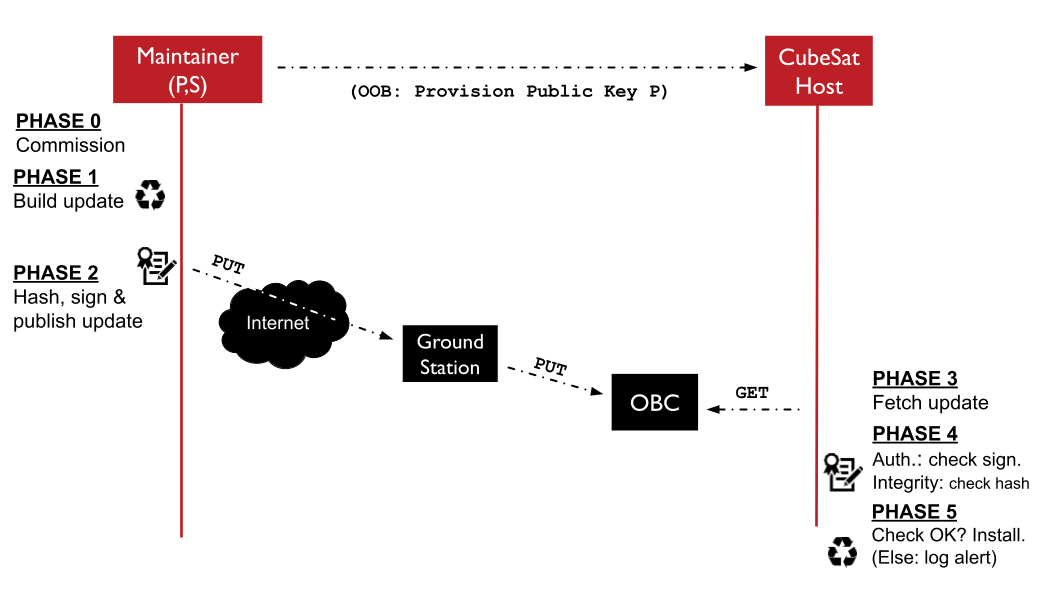
\includegraphics[width=0.5\textwidth]{Figures/CubeSat-Payload-update.png}
    \caption{CubeSat hosted payload secure software update process.}
    \label{fig:phases}
\end{figure}

\subsection{Supporting Network Transport Heterogeneity}
This aspect concerns both \textit{Phase 3.1} and \textit{Phase 3.2} in \autoref{fig:phases}. 

First of all, software updates may be transported over a wide variety of network segments.
\begin{itemize}
\item {\bf Developer-Groundstation segment}: via wired Internet, USB key upload...
\item {\bf Groundstation-CubeSat segment}: via radio links such as UHF, LoRa...
\item {\bf Intra-CubeSat segment}: via bus communication such as CAN/CSP, SPI...
\end{itemize}

Second, paths across the network may vary in complexity.
In the simplest case (typical CubeSat use-case) the end-to-end network path covers only the segment from ground station to the OBC.
In more complex cases involving hosted payloads, not only
must the end-to-end path traverse heterogeneous network segments,
but also: this path may never exist end-to-end at any point in time.
This Delay-tolerant network characteristic is due to power-off periods imposed on CubeSat hosted payloads, 
combined with orbiting CubeSat being out-of-range most of the time via radio w.r.t. available ground stations.
Hence, while in transit across the network, software update data may have to be temporarily cached at some intermediate node along the path.

To cope with this wide variety of scenarios, different solutions may be used at the network, transport and application layers. \todoEB{Add here some short text about what ThingSat does, also hint at exotic things such as ICN?}. 


However, Cubedate does not specify the use of any particular approach at the network, transport and application layers to enable the delivery of software updates across the network.
Cubedate only aims to guarantee end-to-end security properties for the software update binaries delivered over the network.

\subsection{Supporting Updated Software Heterogeneity}
This aspect concerns both \textit{Phase 1} and \textit{Phase 5} in \autoref{fig:phases}. 
Software that must be updated may be of various nature, and size.
(1 )Firmware updates, (2) Mission/configuration files, (3) things like Femto-containers?.

\subsection{Low-power Standardized End-to-End Security}

\todoEB{Describe and motivate here use of of SUIT metadata.}

Using Cubedate and the SUIT standard, software updates for payload hosted on CubeSats mitigate attacks including:

\begin{itemize}
\item {\bf Tampered Software Update Attacks –} An attacker may try to update the IoT device with a modified and intentionally flawed software image. To counter this threat, Cubedate uses digital signatures on a hash of the image binary and the metadata to ensure integrity of both the firmware and its metadata.

\item {\bf Unauthorized Software Update Attacks –} An unauthorized party may attempt to update the IoT device with modified image. Using digital signatures and public key cryptography, Cubedate ensures, that only the authorized maintainer (holding the authorized private key) will be able to update de device.
\end{itemize}

Going beyond simple authenticity and integrity guarantees for software updates delivered over the network, using Cubedate also mitigates other attacks including:
\begin{itemize}
\item {\bf Software Update Replay Attacks –} An attacker may try to replay a valid, but old (known-to-be-flawed) software. This threat is mitigated by using a sequence number. Cubedate uses a sequence number, which is increased with every new software update.

\item {\bf Software Update Mismatch Attacks –} An attacker may try replaying a software update that is authentic, but for an incompatible device. Cubedate includes device-specific conditions, which can be verified before installing a software binary, thereby preventing the device from attempting to use an incompatible software image.
\end{itemize}

\iffalse

\paragraph*{communication protocols}
\paragraph*{software/firmware updates}
\paragraph*{software/configuration updates requirements}

\subsection{Architecture}
\subsubsection{OS}: RIOT
\subsubsection{Network Stack}: COAP/LibCSP/CAN
\subsubsection{Mission Workflow}: mission files
\subsubsection{DevOps Workflow}: SUIT + containers
\paragraph*{SUIT}
\paragraph*{Containerization}
\fi

\section{Cubedate Implementation}
\label{sec:implementation}

\iffalse
SUIT is used in Cubedate payloads as a \textit{Data Delivery Mechanism} bundling
the security properties described in section IV D. The implementation described
next seeks to remain generic to be re-usable in different scenarios while tailored
for the Satellite ThingSat use case.

SUIT state machine running on the deployed device does not need to care about
how this \textit{Data} is delivered or where it will be installed, it just
needs to be handed a \textit{manifest}.

\begin{itemize}
    \item \textbf{Data Resource URI}: a locally (e.g.: mounted USB  device) or remotely
    (HTTP or CoAP endpoint) accessible file.
    \item \textbf{Data Resource Delivery Mechanism}: transport mechanism to deliver SUIT:
    e.g. \{message model, network stack, network interface\}
    bundle, or FileSystem \textit{read/write} functions.
    \textit{manifest} and data resource to the SUIT state machine.
    \item \textbf{Data Resource Installation Storage}: internal or external Volatile or
    Non-volatile storage, e.g. RAM (mission files, FemtoContainers\cite{zandberg2021femto})
    or FileSystem or internal FLASH.
\end{itemize}

As the case where the Data Resource URI points to a locally available is simply a
simplified case, a networked scenario with a URL will be described.

\francisco{PLACE HOLDER FOR A DIAGRAM}
\fi

We implemented Cubedate by extending previous work~\cite{zandberg2019secure} on SUIT support in RIOT, combined with our open source firmware running on the Thingsat payload (also based on RIOT).

\subsection{Intra-cubesat bus communication}

We used \texttt{libCSP} (the library implementing the Cubesat Space Protocol CSP) to provide an easier, socket-like API on top of the raw CAN bus communication channel between the OBC and the payload. More generally, libCSP aims to support the most common serial communication interfaces found on \textit{Satellite} payloads, OBC and components (links such as I2C, RS-232, CAN and wrappers for TAP, ZMQ etc.) 




\subsection{Intra-cubesat bus communication}

\subsection{Intra-Cubesat bus communication}

\subsection{Message Model, Request/Response Semantics}

A \texttt{client/sever} model adequately represents the interactions between the SUIT state
machine (ran in the \textit{payload}) and the Data Resource. In the scope of the
update process the \textit{payload} will act as the client requesting a \textit{manifest}
and sequently the \textit{Data Resource}, but in the global picture it will act
as both \texttt{client \& server}, answering to queries from the OBC or the
ground-segment. ThingSat uses UP \francisco{some info on UP}, a proprietary message
model enabling request-response type interactions, which can be replaced by a
generic \texttt{Request/Response} layer.

\texttt{CoAP} is therefore used because its designed to run on a connection-less transport
and offers little overhead in the exchanged messages as well as support for exchanging
messages larger than the underlying protocols MTU (\francisco{cite block coap}
(4 \texttt{bytes} \texttt{CoAP} header, 0-3 extra \texttt{bytes} for block transmissions).
Using a standard like \texttt{CoAP} allows for simplified integration into \textit{North-bound}
application code, e.g.: \texttt{SUIT} as well as allowing to easily replace the
\texttt{South-bound} network-stack.

Note that a \texttt{Request/Response} approach is not a requirement, but makes
for a clean architecture.

\subsection{Network Stack}

A CubeSat Network will commonly be split into two segments: an in-orbit segment
(OBC \& \textit{payloads}) and a Ground-segment (Ground Station). This motivated
the existence of the \textit{Cubesat Space Protocol CSP} deployed on Satellites
such as Nuts, GomSpace, etc. \francisco{cite}. But recent deployments see CubeSats
as part of larger Network such as LoRaWan \francisco{cite fossa}, and IP based
networks are also present on CubeSats.

\textit{CSP} usage was a requirements specified from SatRevolution as the network
stack to use for ThingSat. Nonetheless this implementation aspired to be agnostic
in design to the network stack, allowing to easily replace it by e.g. an
\texttt{IPV6/UDP} or \texttt{LoRaWAN} stack.

This was done by using a {\bf A generic North-bound interface} called \texttt{sock}
which provides a socket-like API for network stacks. Although designed for IP,
it can be wrapped around CSP if care is taken to handle addressing.

\subsection{Communication Bus}

\texttt{LibCSP} and \textit{CSP} support several physical layers such as CAN, I2C,
RS-232, network interfaces wrappers also exist for TAP, ZMQ, and can be easily
extended to cover the radio link between the \textit{Satellite} and
\textit{Ground-Segment}. The physical layers supported are not random, they match
the most common serial communication interfaces found on \textit{Satellite}
payloads, OBC and components. Ethernet is also commonly available  but prohibitive
in most microcontrollers based use-case because of its high power consumption.
\francisco{add some details on CAN?}

CAN was used since it provides an extremely robust, simple and efficient,
widely proven in the automotive, flight and space industry.

\subsection{Operating System: RIOT}

RIOT is a general-purpose OS designed for small IoT devices based on micro-controllers.
It provides with blah blah..

\subsubsection{Integrating LibCSP and RIOT}

Details on the integrations work, learned lessons and sufferings.

\subsection{Continuous Integration \- Collaborative Platform}

The CubeDate architecture was implemented on ThingSat (using UP instead of CoAP).
A Continuous Integration collaborative platform mimicking the update workflow described
in section \francisco{section?}. This consist on a minimal implementation of the
\texttt{OBC} - \texttt{payload} interactions.

The \texttt{OBC} can be ran on RIOTs \texttt{native} platform with a mounted
FileSystem or on any RIOT \texttt{board} with an `sdcard` slot or adapter.
\textit{manifests} and matching \textit{Data-Resources} can be pushed to the
\texttt{OBC} which in its turn acts as a \texttt{CoAP} file-server.

The Payload can run on RIOTs \texttt{native} platform or on any \texttt{RIOT}
\texttt{board}. Different \textit{Data-Resources} can be delivered to RAM,
External NVM or internal NVM (FLASH), simulating delivery of mission files,
firmware updates or other.

Both \texttt{OBC} and \texttt{payload} run over \texttt{LibCSP} over CAN. If
using \texttt{native} \texttt{SocketCAN} is used to create virtual can
devices.

\francisco{Place Holder of Diagram of the CI}

The developments related to this paper where in release in open-source form for
the benefit of CubeSat and RIOT communities and can be found at.


\section{Cubedate Evaluation and Discussion}
\label{sec:evaluation}

%The analysis of the implementation was two-fold, first we evaluate how the SUIT based architecture fitted the CubeSat and CubeSat hosted payload use case. Second, we discuss possible modifications to the workflow, architecture and protocols.

%\subsection{Evaluation}

In the following, code measurements where generated compiling with ARM GCC 10.2.1,
optimized for code size. As code base, we used RIOT release 2022.01 and SUIT configured with ed25519 digital signatures provided by the C25519 crypto library as backend (which has small footprint as shown in prior work~\cite{zandberg2019secure}).

\subsubsection{Memory Footprint Overhead}

To evaluate the RAM and Flash footprint of our Cubedate implementation, we apply it to the Thingsat use-case, compiled for the hosted payload hardware described in \autoref{sec:thingsat-hw} (based on a Cortex-M microcontroller).  

In \autoref{tab:footprint} we compare the RAM and Flash memory requirements for a Thingsat firmware without/with Cubedate-compliant secure software updates.
We observe that Cubedate requires a memory budget of $\sim$4kB of RAM and $\sim$19kB of Flash, which represents roughly a 10\% increase in the total RAM and Flash memory budget for Thingsat.

\subsubsection{Network Transfer Overhead}
On the UHF/VHF link at 1kb/s, the additional network transfer time induced by the Cubedate firmware size overhead (19kB) is roughly 15 seconds. This overhead is reasonable, but not negligible keeping in mind that a connection to the cubesat is segmented in time windos of $\sim$ 300 seconds.

Next, in \autoref{tab:footprint} we look in more details at the metadata (SUIT manifest) used to secure Cubedate software updates for Thingsat.
As we can see, the metadata including all CBOR/COSE formating, digests (SHA256 hashes) and autentication data (ed25519 signature) amounts to $\sim$330Bytes. The metadata overhead thus incurs negligible overhead (+0,15\%) in case of a Thingsat firmware update (of size 200kB on average, recall \autoref{sec:thingsat-update-req}). However, in case of a smaller software update such as updating a mission scenario (average size 700Bytes) the overhead of adding Cubedate metadata is significant (almost +50\%). 
Nevertheless, on the UHF/VHF link at 1kb/s, this overhead remains negligible in terms of additional network transfer time.

\iffalse

architecture we evaluate them
in two configurations, furthermore we categorize the different components to
distinguish the SUIT endured overhead

\begin{itemize}
    \item \textbf{ThingSat} refers to the ThingSat payload application with no
    software updates support
    \item \textbf{CubeDate} implementation of the CubeDate architecture on the
    ThingSat payload
    \item CAN (Controller Area Network) stack as well as low level interface
    \item Crypto includes all cryptographic algorithms such as digest algorithm, digital
    signature, ECC and bignum, as well as pseudo-random numbers generator
    \item CoAP protocol library (CoAP endpoint stack excluded)
    \item CSP (Cube Sat Protocol) network stack
    \item LoRa GW includes the sx1302 driver as well as the gateway code
    \item SUIT englobe all components enabling retrieval and installation of suit data
    (fw or other), this include e.g. the CoAP endpoint stack.
    \item Firmware: application specific code related to the CubeSat Payload excluding
    the LoRa gateway
\end{itemize}

The flash memory footprints (total and broken down per component) are shown in
\autoref{tab:footprint}. It can be seen that the overhead of Cubedate for ThingSat
is of \~4Kbytes of RAM and \~19Kbytes of flash.
\fi


\begin{table}[t]
\begin{adjustbox}{width=0.8\columnwidth,center}
    \centering
    \includestandalone[width=1\columnwidth]{Figures/texfigs/memory_footprint_table}
\end{adjustbox}
\caption{Cubedate implementation: memory footprint in Bytes.}
\label{tab:footprint}
\end{table}

\subsection{Discussion \& Perspectives}

\subsubsection{Network Stack Simplification \& Standardization}
The use of CSP was mandated by the cubesat operator. CSP was designed for cubesats with legacy (8-bit) microcontrollers as an ultra-low footprint equivalent of the IP protocol stack.
However, on modern (32-bit) microcontrollers such as used in ThingSat, we argue that using CSP is questionable: an alternative based on more widely spread standards seems possible for the same "price". For example, RIOT's default low-power IPv6 (6LoWPAN) stack used with static routing has a RAM/Flash footprint that is comparable or smaller w.r.t libCSP. This stack could run direcly on the CAN bus or on LoRa (see 6loCAN~\cite{wachter20206locan01} and SCHC~\cite{rfc8724}).

\iffalse
In fact, taking as base
 CubeSat sub-systems developers the same features as an
TCP/IP stack without the overhead of the IP header, allowing to run on constrained
systems with under 4kB of RAM. Unless running on this kind of very constrained
devices using CSP can be contested. A minimal CoAP server example running on
LibCSP or RIOTs default IPv6/UDP network stack (GNRC) yields similar numbers of RAM/Flash
usage: 10KB\/30KB (CSP) vs 8KB/31KB (GNRC). Optimal compression of an Ipv6 header
can shrink the size from 48bytes to 4Bytes, comparable to CSP2.0 3Bytes header.
Furthermore  6loCAN\cite{wachter20206locan01}, SCHC\cite{rfc8724}, allow to
optimize IPv6 for CAN-BUS or LoRa network. What is gained in simplicity is eventually
lost by using a not standard network stack, i.e. using standard application
layer protocols.
\fi

\begin{table}[t]

\begin{adjustbox}{width=0.5\columnwidth,center}
    \centering
    \includestandalone[width=1\columnwidth]{Figures/texfigs/manifest_overhead_table_simplified}
\end{adjustbox}
\caption{Cubedate implementation: SUIT metadata overhead.}
\label{tab:manifest-overhead}
\end{table}

\subsubsection{SUIT Authentication}

SUIT relies on COSE for authentication, with digital signatures being the most
used method. A viable alternative for CubeSat maybe to instead use a tagged Message
Authentication Code (MAC). This will reduce the size of \textit{Authentication} block
\ref*{tab:manifest-overhead} from 64Bytes to 16Bytes or 8Bytes if using HAMC-256/128
or HMAC-256/64. This would also save Flash since as seen in~\cite{zandberg2019secure}
the ed25519 library accounts for roughly 75\% of the crypto flash budget, while HMAC-256
re-uses sha256 code, and adds an overhead of ~1Kbyte. The requirement for a shared secret
might be an acceptable compromise since attackers gaining physical access to the
in-orbit device is unlikely.

\subsubsection{SUIT Manifest Overhead}

In space communication transferring data is costly, reducing the Manifest
overhead~\ref{tab:manifest-overhead} for mission files transfers is highly
desirable. This can be done by using \texttt{COSE\_MAC0\_tagged} instead of
\texttt{COSE\_SGN0\_tagged} (-56Bytes) and integrating the payload into the
manifest (-64Bytes from the URI), reducing the manifest size to 162Bytes,
effectively reducing the overhead to \~23\%.


\section{Lessons Learned}



\section{Next Steps \& Future Work}
\label{sec:futurework}

\paragraph*{RIOT/SUIT differential firmware updates}
\paragraph*{Business logic containerization}

\section{Conclusion}
\label{sec:conclusion}


\section*{Acknowledgment}

\bibliographystyle{IEEEtran}
\bibliography{biblio}

\end{document}
